\chapter{nD-Laplace}
In this chapter, we delve deeper into geo-indistinguishability and the various mechanisms that work with it, \added{and aim to provide the theoretical foundation for research questions 1, 2 and 3.}
We also explain the theory behind the nD-Laplace mechanism and how we modify it and apply it for clustering.
%This explanation is build-up out of several sections, each dedicated to 2, 3, and n-dimensional data.
Because we frequently discuss 2, 3, and dimensional data in our thesis, we decided to prefix the respective Laplace method with this information.
Therefore, for the rest of the thesis, we use the following names:
\begin{enumerate}
  \item 2D-Laplace: This refers to the planar Laplace mechanism \citep{DBLP:journals/corr/abs-1212-1984}.
  \item 3D-Laplace: This refers to the spherical Laplace mechanism \citep{9646489}.
  \item nD-Laplace
\end{enumerate}
\replaced{The theory, mechanism, and data truncation are explained for each section. In addition, an explanation is provided when a section relates directly to a research question.}{For each mechanism, we explain the equation for \gls{gi}, the mechanism, and the data truncation.}

\printnomenclature

%
\newglossaryentry{X}
{
  type=genericmath,
  name={$\ensuremath{X} $},
  description={Set of locations for a user. ($R^2$)},
}
\newglossaryentry{Z}
{
  type=genericmath,
  name={$\ensuremath{Z} $},
  description={For every $x \in X$ a perturbed location $z \in Z$ is reported.},
}
\newglossaryentry{privacy level}
{
  type=genericmath,
  name={$\ensuremath{l} $},
  description={Privacy level},
}
\newglossaryentry{radius}
{
  type=genericmath,
  name={$\ensuremath{r} $},
  description={Radius},
}
\newglossaryentry{Epsilon}
{
  type=genericmath,
  name={$\ensuremath{\epsilon} $},
  description={Defined as $\epsilon = l/r$},
}
\newglossaryentry{theta}
{
  type=genericmath,
  name={$\ensuremath{\theta} $},
  description={Angle},
}

\newpage
\section{2D-Laplace}
The idea of \gls{gi} was introduced to address the issue of privacy and location data \citep{DBLP:journals/corr/abs-1212-1984} (See Equation \ref{algo:2d-geo-indistinguishability}).
It offers an alternative approach for achieving (local) differential privacy for geographical data (latitude/longitude).
The mechanism achieves this by locally adding noise to the location before sending it to a location-based system (LBS).
This section starts with an introduction to mathematics, and for each of the different subsections, we visualize and explain open challenges and theoretic for applying them for clustering.
%\glsaddall
%\leading{10pt}
%\printglossary[type=genericmath, nonumberlist]
%The other symbols can be found in section \ref{section:dp}.
\subsection{Planar and polar Laplace}
In Section \ref{theory:geo-indistinguishability}, we provided an explanation of the concept of \gls{gi}. 
Additionally, we introduced the notion that when a point $x_0 \in X$ serves as the center of a range $r$, a point $z \in Z$ is generated using a noise function \citep{DBLP:journals/corr/abs-1212-1984}. The objective here is to ensure that when the actual locations are $x_0$ and $x_0'$, their divergence is limited to at most $e^{-\epsilon \cdot d(x_0, x_0')}$. This characteristic aligns with the Laplace distribution, which the "planar Laplace" mechanism leverages.
Furthermore, it is worth noting that the "planar Laplace" mechanism is an adaptation of the Laplace distribution designed to accommodate distances in a 2-dimensional space \citep{DBLP:journals/corr/abs-1212-1984}. For clarity, we will refer to this method as "2D-Laplace" from this point forward.

The distance method $d(\cdot, \cdot)$ is a method to calculate the Euclidean distance between two points.
Recalling the definition of Laplace, this method $|x-x'|$ is replaced by the distance metric.
Given the actual location $x_0 \in X$, the \gls{pdf} of the noise mechanism on any other point $z \in Z$ is provided as \citep{DBLP:journals/corr/abs-1212-1984}: 
\begin{equation}
  D_\epsilon(x_0)(z) = \frac{\epsilon^2}{2 \cdot \pi}e^{-\epsilon \cdot d(x_0, z)}
  \label{eq:polar-laplace-pdf}
\end{equation}
The method works for Cartesian coordinates but was modified to support polar coordinates by including $\theta$.
So each polar coordinate is reflected as $(r, \theta)$, where $r = d(x_0, z)$ around point $x_0$.
This idea is visualized in the following figure:
\begin{figure}[H]
  \includesvg[scale=1]{TheorethicalFramework/ND-Laplace/Images/polar-laplace.svg}
  \centering
  \caption{Representation of the generated $(r,\theta)$ and original point $x_0$.}
  \label{figure:parea}
\end{figure}
Next we show in detail, how to generate the polar coordinates $(r, \theta)$. \newline
\textbf{Calculating $r$:}
The $r$ is randomly selected based on a distribution $R$ \citep{DBLP:journals/corr/abs-1212-1984}: 
\begin{equation}
    D_{\epsilon, R}(r) = \int^{2\cdot \pi}_0 \ D_\epsilon(r, \theta) \ d\theta = \epsilon^2 \ r \epsilon^{-\epsilon \cdot r}
    \label{2d:generate-r}
\end{equation}
Where the $r$ is selected randomly on the area of the circle. 
Next, it can be randomly drawn by inverting the \gls{cdf} for the Laplace distribution \citep{DBLP:journals/corr/abs-1212-1984}:
\begin{equation}
  C{_\epsilon}{^{-1}}(p) = - \frac{1}{\epsilon}(W_-1 (\frac{p - 1}{e}) + 1)
  \label{eq:lambert_w_1}
\end{equation}
For this equation, the Lambert $W$ function is used. This function consists of two different branches \citep{corless_lambertw_1996}. This means the value of $W_0(x)$ is always positive, while $W_{-1}(x)$ is always negative. The Lambert w function (also called the product logarithm) is defined as $W(x)e^{W(x)} = x$ \citep{lehtonen_lambert_2016}.
The purpose of the Lambert W function is to invert the \gls{cdf} of the Laplace distribution to generate random noise for one of the coordinates ($r$) using the random value of $p$. It draws the $r$ which will be bounded by the $W_{-1}$, this is very useful for drawing the random planar noise \citep{corless_lambertw_1996}.

\textbf{Calculating $\theta$:}
The other variable ($\theta$) is defined in a similar way \citep{DBLP:journals/corr/abs-1212-1984}: 
\begin{equation}
    D_{\epsilon, \Theta}(\theta) = \int^\infty_0 D_\epsilon(r, \theta) \ dr = \frac{1}{2 \cdot \pi}
    \label{2d:generate-theta}
\end{equation}
To visualize the data, it is necessary to convert the polar coordinates for $(r, \theta)$ to Cartesian coordinates $z = (x, y)$.
This conversion is described as step 4 of the planar Laplace algorithm \citep{DBLP:journals/corr/abs-1212-1984} and visualized using figure \ref{figure:geo}.
\begin{figure}[h]
    \centering
  \includesvg[width=0.8\textwidth]{TheorethicalFramework/ND-Laplace/Images/polar-laplace-to-planar.svg}
  \centering
  \caption{Representation of converting the polar coordinate $(r, \theta)$ to a perturbed point $z = (x, y)$.}
  \label{figure:geo}
\end{figure}

\newpage
\subsection{Truncation} \label{theory:truncation}
After adding the noise to the data, it cannot be ensured the data is within the original domain (figure \ref{figure:truncation-2d}).
If this is not the case, the data is easily distinguished by an unwanted adversary \citep{DBLP:journals/corr/abs-1212-1984,9646489}.
The truncation is an essential part of the mechanism to ensure the data is contained within the domain of the original data $X$. The following example shows two different original points $x_0$ and $x_0'$, where $z$ and $z'$ are being remapped to be within the domain:
%We assume a user has a set of data points with a range of [-1, 1].
\begin{figure}[H]
\centering
  \includesvg[width=1\textwidth]{TheorethicalFramework/ND-Laplace/Images/remapping.svg}
  \caption{Representation of truncation of data points for 2-dimensional Laplace mechanism.}
  \label{figure:truncation-2d}
\end{figure}
%A solution was described by Andres et al. in step 5 of the Laplacian mechanism for 2D space \citep{DBLP:journals/corr/abs-1212-1984}.
%A viable solution is to create a grid around the diameter of the set of points $X = R^2$ that belong to the user \citep{DBLP:journals/corr/abs-1212-1984}.
This approach was introduced by Andres et al. to remap a perturbed point $z$ to the closest point in $G$ \citep{DBLP:journals/corr/abs-1212-1984}.
Here, $G$ is a grid with sides $u$ and $v$, such that $u \leq v$.
%Although this approach remaps data within the original domain of $X$, it is not guaranteed it preserves \gls{gi} anymore.
Let the below equation be the collection of probabilities for a point $z$ being remapped to a closest point in $G$:
\begin{equation}
  R(z) = \{ \ y \in R^2 \ | \ \forall z' \in G \cdot d(y, z') \leq d(y, z') \ \}
  \label{eq:grid-probability}
\end{equation}
The original \gls{gi} definition contains $K$, which is the probability of $z$ being reported as $x_0$ (See Equation: \ref{theory:geo-indistinguishability}).
However, this probability is no longer guaranteed because $z$ can also be part of $G$ \citep{DBLP:journals/corr/abs-1212-1984}.
Hence the probability is now $R(z) = G \cap A$. Where $A$ is a set of acceptable datapoints.\newline
So, $R(z)$ has a different shape depending on the distance $x_0$ and $z$ (ergo, it depends on the grid unit $v$ or $u$). This is due the step units of $G$ stay the same, while the distance $r$ grows \citep{DBLP:journals/corr/abs-1212-1984}.

To overcome this issue, Andres et al. propose a way of calculating $\epsilon'$, depending on the step-unit $u$. \citep{DBLP:journals/corr/abs-1212-1984}.
They proved this and provided theorem 4.1 \citep{DBLP:journals/corr/abs-1212-1984}:
\begin{theorem}[Discretization 2D-Laplace]
  Assume $r_{max} < \frac{u}{\delta_{\theta}}$, and let $q = \frac{u}{r_{max}}\delta_{\theta}$. \\ Let $\epsilon$, $\epsilon' \in R^+$ such that \\
  $\epsilon' + \frac{1}{u}ln \frac{q + 2 e^{\epsilon'u}}{q - 2 e^{\epsilon'u}} \leq \epsilon$ \\
Then $K_{\epsilon'}$ provides $\epsilon$-geo-indistinguishability within the range of $r_{max}$. \\ 
  Namely, if ${d(x_0, z), d(x'_0, z) \leq r_{max}}$ then: \\
  $K_{\epsilon'}(x_0)(z) \leq e^{\epsilon d(x_0, x'_{0})} K_{\epsilon'}(x'_{0})(z)$.
  \label{theorem:discretization}
\end{theorem}
Where $x_0$ and $x_0'$ are two different original points for which the noise is generated. 
Here, $\delta_{\theta}$ is the machine's precision, which is the hardware precision of the GPS-location in the context of geographical data. We will omit this in our research, but still provide the full theorem nonetheless.
The theorem states that $\epsilon'$ is the additional noise needed to satisfy \gls{gi} with the introduction of discretization.
%Then, the final step is truncation based, which is based on the discretization \citep{DBLP:journals/corr/abs-1212-1984}.
It is sufficient to take $r_{max}$ as $diam(A)$, which is the diameter of the set of points $A$ if it satisfies theorem \ref{theorem:discretization} \citep{DBLP:journals/corr/abs-1212-1984}:
So, $r_{max}$ is the maximum distance between points in $A$, which is the area where geo-indistinguishability can be guaranteed \citep{9646489}.
%This idea was later improved by Chatzikokolakis et al., introducing an optimized way of remapping \citep{chatzikokolakis_efficient_2017}.
%The algorithm uses the Bayesian rule to minimize the loss of utility while remapping the data.
%Instead of remapping to the closest point, it remaps to a location where the loss is minimal.
%To decrease the performance impact of this algorithm, it is possible only to consider a specific region around the perturbed point $z$.
%The disadvantage of this method is the need for a prior set of data points to calculate the optimal remapping.
%It does not work for new users and extends the training period.
\subsection{Final mechanism}
Finally, we provide as means of a summary the final algorithm for the Laplace mechanism for 2D space
\begin{algorithm}[H]
  \caption{Full mechanism for perturbing training data for 2D-clustering using planar/2D-Laplace \citep{DBLP:journals/corr/abs-1212-1984}}\label{alg:rq1}
  \begin{algorithmic}
    \Require $x \in X$  \Comment 2D array of points \\
    $\epsilon$ \Comment should satisfy Theorem \ref{theorem:discretization}
    \Ensure $z \in Z$ \Comment 2D array of perturbed points
    %\State $r = \frac{\sigma}{2}$ \Comment formula 4.1
    %\State $\epsilon = \frac{l}{r}$ \Comment Calculating privacy budget \citep{DBLP:journals/corr/abs-1212-1984}
    \State $x_{min} \gets min(X)$
    \State $x_{max} \gets max(X)$
    \State $Z \gets []$
    \For{$point_i \in X$}
    \State $\theta \gets [0, \pi2]$       \Comment Random noise for $\theta$
    \State $p \gets [0, 1]$
    \State $z_i \gets C{_\epsilon}{^{-1}}(p)$       \Comment formula 3.2
    %\State $z_i \gets T(x_{min}, x_{max}, point_i, z_i)$ \Comment algorithm 1.
    \State $x_{perturbed} \gets point_{i_x} + (z_{i_x} * \cos(\theta)) $ \Comment add noise to x-coordinate
    \State $y_{perturbed} \gets point_{i_y} + (z_{i_y} * \sin(\theta)) $ \Comment add noise to y-coordinate
    \State append $x_{perturbed}, y_{perturbed}$ to Z
    \EndFor
    \State \Return Z
  \end{algorithmic}
  \label{alg:2d-laplace}
\end{algorithm}
\newpage
\section{3D-Laplace}
\todo[inline]{Is considered for research question 3}

\newpage
\section{nD-Laplace}
As mentioned in the previous chapter, the paper introduced by Min et al. can handle 3-dimensional data.
A small recap: a point $(r, \theta, \psi)$ gives us the three coordinates of a location on the 3-dimensional sphere.
An important property is that these coordinates can be generated separately \citep{DBLP:journals/corr/abs-1212-1984, 9646489}.
The $r$ gives us the radius or distance from $(\theta, \psi)$ to the center of the sphere \footnote{https://mathworld.wolfram.com/SphericalCoordinates.html}.
So, instead of having just these two coordinates, we can extend this to n-dimensions by considering an n-hypersphere \citep{fernandes_generalised_2019, 9646489}.
The theorems for \gls{gi} are extended by Fernandes et al. to support n-dimensional data:
%To this end, in addition to points $\theta$ and $\psi$, we consider $\theta \in S^n$, where $S$ is a unit hypersphere.
\begin{theorem}
  Let $d_x$ be a pseudo-metric on $X$ and let $K: X \rightarrow Z$ be a mechanism satisfying $\epsilon-d_x-privacy$. \\
  $K(x)(Z) \leq e^{\epsilon \cdot d_x (x, x')} \cdot K(x')(Z), \forall x, x' \in X, Z \subseteq X$.
  \label{theorem:nd-laplace}
\end{theorem}
This theorem extends $\epsilon$-geo-indistinguishability to $\epsilon-d_x$-privacy as a more general notion of distinguishability \citep{fernandes_generalised_2019}:
Here, $d_x$ is a pseudo metric which was provided by Chatzikokalakis et al. as elastic privacy definition for location privacy \citep{chatzikokolakis_constructing_2015}. For the use with the Euclidean distance, the privacy definition is defined as $d_{euc}$. Due to the flexibility of $d_x$ the theorem \ref{theorem:nd-laplace} also holds for $d_{euc}$.  Furthermore, $\epsilon-d_{euc}$ provides the same privacy definition as geo-indistinguishability \citep{chatzikokolakis_constructing_2015}.
Therefore, $d_{euc}$ is adopted by this thesis from now on, to be used for applying it for non-geographical data to establish a more general notion of privacy. \newline

The 2D-Laplace mechanism is referenced as a plane, and the coordinates can be generated separately as $(r, \theta)$ \citep{fernandes_generalised_2019,DBLP:journals/corr/abs-1212-1984}.
Hence, generating the nD-variant can be seen as generating multiple $(r, \theta)$ pairs \citep{fernandes_generalised_2019}.
Where $r$ is the radial distance from the origin $x_0$ and $\theta$ is the angle randomly selected from a unit hypersphere.
The selection of $r$ is according to the Gamma distribution, with shape $n$ and scale $\delta > 0$ \citep{fernandes_generalised_2019}:
\begin{equation}
  Gam^n_\delta(r) := \frac{r^{n-1}\cdot^{-\frac{r}{\delta}}}{\delta^n(n-1!)}
  \label{eq:generate_r_for_nd_laplace}
\end{equation}
Then, $\theta$ is drawn from a uniform distribution of a unit hypersphere $S$ \citep{fernandes_generalised_2019}:
\begin{equation}
  Uniform^n(\theta) := \frac{\gamma(\frac{n}{2})}{n \cdot \pi ^{\frac{n}{2}}}
  \label{eq:generate_theta_for_nd_laplace}
\end{equation}
Where $\gamma(a) = \int^\infty_0 x^{a-1} \cdot e{-x} \cdot d \cdot x$ is the gamma function \citep{fernandes_generalised_2019}.
This approach is similar to the other variants of the Laplace mechanism.
Only now, we select points from an $n$-dimensional hypersphere  \footnote{https://mathworld.wolfram.com/SpherePointPicking.html} instead of a unit sphere \ref{eq:3d-laplace-2}. \newline

In the next step, the spherical coordinate representation is converted to Cartesian coordinates \citep{fernandes_generalised_2019}:
It is comparable to the way it was done in the previous chapters; however, as there are an $n$-amount of angles, the equation is repeated and slightly different.
The formula is provided by Fernandes et al. to convert $r$ to spherical coordinates \citep{fernandes_generalised_2019}:
\begin{align}
  x_1 = r * cos (\theta_1)                                          \\
  x_2 = r * sin (\theta_1) * cos (\theta_2)                         \\
  x_{n} = r * sin(\theta_1) … sin(\theta_{n-2}) *cos (\theta_{n-1}) \\
  x_n = r * sin(\theta_{n-1}) * sin(\theta_{n-2}) * sin(\theta_{n-1})
  \label{eq:nd-laplace-cartesian}
\end{align}

The combination of sections 1 and 2 of this chapter provides a good overview of the solution using a similar image as the 2D and 3D variants (figure \ref{fig:nd-laplace-overview}).
\begin{figure}[H]
   \centering
  \includesvg[width=0.8\textwidth]{TheorethicalFramework/ND-Laplace/Images/nd_laplace}
  \caption{Overview of the nD-Laplace mechanism}
  \label{fig:nd-laplace-overview}
\end{figure}
\todo[inline]{Update image with other notation and add explanation}
\newpage
\subsection{Privacy versus utility} \label{theory:privacy-utility-nd}
When we specifically look at the \(uniform^n(\theta)\) function (see Equation: \ref{eq:generate_theta_for_nd_laplace}), the \(\theta\) can be generated \(n\)-times, but this has some limitation \footnote{\url{https://mathworld.wolfram.com/Hypersphere.html} \label{footnote:hypersphere}}.
The value of \(\theta\) decreases after the $\approx 7$ dimensions have been reached \citep{wells_penguin_1997}. Subsequently, the hyper-surface area reaches a maximum, so the value of $\theta$ decreases towards 0 \footnote[\ref{footnote:hypersphere}].
This behaviour is illustrated in the following figure:
\begin{figure}[H]
\centering
  \includesvg[width=0.8\textwidth]{TheorethicalFramework//ND-Laplace//Images/HypersphereArea_900.svg}
  \caption{Illustration of the decreasing volume while increasing the number of dimensions \footnote{\url{https://mathworld.wolfram.com/Hypersphere.html}.}
  \label{fig:curse-of-dimensionality}
\end{figure}
As can be seen in the image, the amount of volume starts to decrease after the 7 dimensions . From this, it can be inferred that the value of  $\theta$ will also decrease. 
The consequence of this behavior is that the final noise decreases for higher dimensions. This will result in the possibility that utility increases in higher dimensions, but privacy decreases.

\newpage
\subsection{Grid-remapping}
In the previous sections, we introduced the 2D, 3D, and nD Laplace mechanisms.
The current section will be used to formalize nD-Laplace with grid-remapping (disretization \& truncation) and introduce modifications to improve the mechanisms for clustering for n-dimensional data.

\subsubsection{Discretization and truncation} \label{theory:nd-laplace-truncation}
To recall the working of 2D and 3D-Laplace remapping, we give a short summary of these two sections. The discretized 2D version operates on a plane and approximates on a grid $G$, while the 3D version works in a sphere and approximates the data using a cuboid grid  $G_C$.
Given a set of perturbed points $Z$ we can truncate the points that are outside the domain by remapping them to points within $G$ ($Z = X \cap G$) \citep{DBLP:journals/corr/abs-1212-1984}.
Here, $X$ represents other non-private data points reported locally by the same user.
The following part aims at extending the theorems for 2D and 3D-Laplace for discritezation and truncation to n-dimensions. \newline

The theorems for 2D (See Theorem \ref{theorem:discretization}) and 3D-Laplace (See Theorem \ref{theorem:3d-discretization}) include a device precision. 
This variable is the hardware precision of a GPS provided by the user's device (e.g. a mobile phone). 
For the purpose of clustering, we omit this for the formulation of truncation with n-dimensions.

We extend the reasoning of Min et al. behind extending 2D-Laplace to 3D-Laplace as this applies to nD-Laplace as well.
Let $v > w > h$ be a cuboid grid $G_c$, equal to the one provided by Min et al \citep{9646489}.
We are be-able to extend this by providing a hypercube ($n$-cube) with n-dimensions denoted as $G_n = u_1, u_2, u_3 ... u_n$. This $n$-cube has $2^n$ sides, but can essentially be seen as a generalization of a 3-cube to $n$-dimensions \footnote{https://mathworld.wolfram.com/Hypercube.html}.

However, An issue arises with the definition of the grid-units, where Min et al. and Andres et al. both consider the possibility of unequal grid-units, for the purpose of generalisation \citep{9646489, DBLP:journals/corr/abs-1212-1984}. 
But for a $n$-cube this is generalisation is harder to justify, because the are $2^n$ possible sides to consider.
For this reason, we define $v, w, h = u_1$. We choose $u_1$, but in general this can be any given value $u \in G_n$.

Another important property, is the maximum diameter defined as $r_M$ \citep{9646489}.
This property can also be converted to support n-dimensions, by calculating the diameter of $G_n$.
This is the maximum distance between any pair of nodes \citep{HARARY1988277}. \newline
The Euclidean distance diameter is defined as:
\begin{equation}
  d_{euc}(G_n) = r_H = \sqrt{n}
\end{equation}

Where, $n$ is the number of dimensions.
\newpage
Finally, we are be-able to establish our own theorem for the discretization and truncation of nD-Laplace:
\begin{theorem}
  Assume $u$ to be a side length, Let $G_u$ be an $n$-dimensional hypercube of $u$ size, Let $r_H < u$ and let $w = \frac{u^2}{r^2_H \cdot sin (\theta)} > \frac{u}{r_H}.$ Let $\epsilon, \epsilon' \in R^+$ such that \\
  $\epsilon' + \frac{1}{u} ln \frac{w + n \cdot e^{\epsilon' \cdot u}}{w - n \cdot e^{\epsilon' \cdot u}} \leq \epsilon$ \\
  Then $K\epsilon'$ satisfies $\epsilon$-geo-indistinguishability within range
  of $r_H$. That is to say, if $d_n(x, z)$ and $d_{euc}(x, x') \leq r_H$ then,
  $K(x)(z) \leq e^{\epsilon \cdot d_{euc} (x, x')} \cdot K(x')(z)$ forall $x, x' \in X, z \in Z$ \citep{chatzikokolakis_constructing_2015}
\end{theorem}
Since we specify the hypercube to have equal sides of $u_i$, we are be-able to simplify the theorem.
%We use the proof provided by Min et al. in some extend by satisfying preliminary variables \citep{9646489}.
By satisfying the conditions for $r_H$ and $u$, we use the proof provided for 3-dimensions and use it for $n$-dimensions \citep{9646489}.
If we select a $u$ smaller then the max diameter $r_H$, we can satisfy $d_{euc}(x_n, x0) < r_H < u$. Which is according to the proof provided by Min et al.
Moreover, $w = \frac{u^2}{r_H^2 \cdot sin(\theta)} > \frac{u}{r_H}$ is also satisfied as the sizes of $G_n$ are equal.
Given that these pre-conditions apply, we can reuse the proof from 3-dimensions for n-dimensions. \newline

The utility of this method depends on the number of grid cells in $G_n$ since a smaller distance will result in more frequent mapping to the surface of the grid.
When $\epsilon$ is very low (resulting in $z$ being much farther away from $x_0$), data points have a higher likelihood of mapping to map to the grid surface 
(as seen in \ref{fig:3d-laplace-noise}, \ref{fig:3d-laplace-example}). 
While increasing the number of grid cells might enhance utility, it also leads to a notable rise in space complexity. 
Moreover, as the number of dimensions grows, the count of grid cells increases quadratically.

\subsubsection{Optimization}
To make grid-remapping practically possible with n-dimensions, the data structure has to be more efficient to search spatial data. For this purpose, we adopt the idea proposed by Chatzikokolakis et al. of using a kd-tree to search the grid efficiently \citep{chatzikokolakis_efficient_2017}.
Their research describes the theoretical utilization of a kd-tree for searching nearby points for a given point.
For this reason, we aim to apply this practically by using a kd-tree for the following tasks:
\begin{enumerate}
  \item Finding nearby points for $q \in G_c$ (Section: \ref{theory:grid-remapping}).
  \item Finding nearby points for $x \in X$ and $z \in Z$ (Section: \ref{theory:optimal-remapping}).
\end{enumerate}
The usage of kd-tree does not impact any privacy guarantee provided in the previous section. It is just a more efficient way of searching in n-dimensional spatial structures. Also, for visualization purposes, this section will primarily focus on 2D data. \newline
The next section explains the concept and underlying idea of kd-trees.
Then, we delve into its application for grid remapping.
Finally, we expand this to a practical application with nD-Laplace.
\newpage
\subsubsection*{Kd-trees} \label{theory:kd-trees}
A kd-tree algorithm can search a grid for nearby points \citep{bentley_multidimensional_1975}.
It can do so by recursively splitting the grid into a binary tree to search for grid coordinates \citep{washington_k-d_2002}.
In addition, it preserves spatial information of the data so it can be utilized to find nearby points using Euclidean distance (nearest neighbor search).
The following example provides an idea of how this works (Figure \ref{fig:kd-tree-theory}):
\begin{figure}[H]
  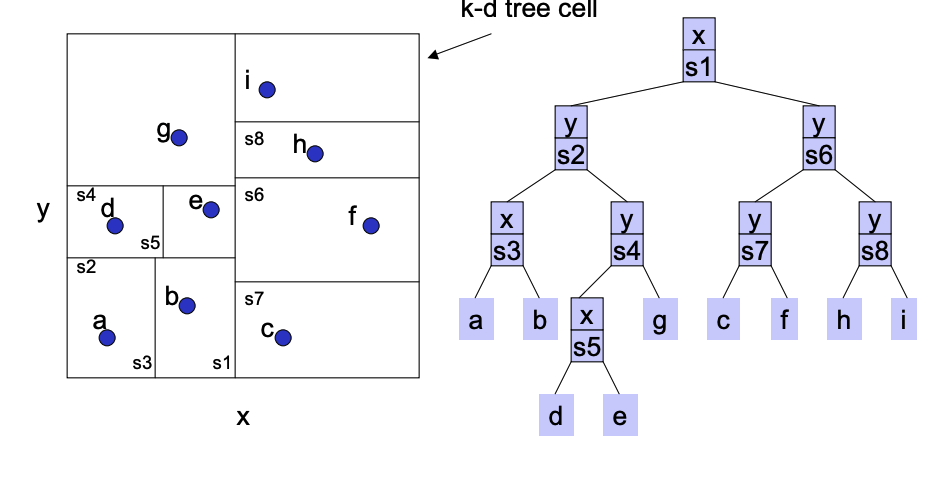
\includegraphics[width=0.8\textwidth]{TheorethicalFramework/ND-Laplace/Images/kd-tree-part1.png}
  \caption{Representation of constructing a kd-tree with 2 dimensions \citep{washington_k-d_2002}.}
  \label{fig:kd-tree-theory}
\end{figure}
Take, for example, the 2D Laplace algorithm that utilizes a plane (left side).
The data points can be divided based on their x and y coordinates.
Each coordinate becomes a node in the binary tree, and the grid is divided based on these splits.
The binary tree allows us to search the grid efficiently.
An example of this is provided in the following image (Figure \ref{fig:kd-tree-searching-theory}):
\begin{figure}[H]
  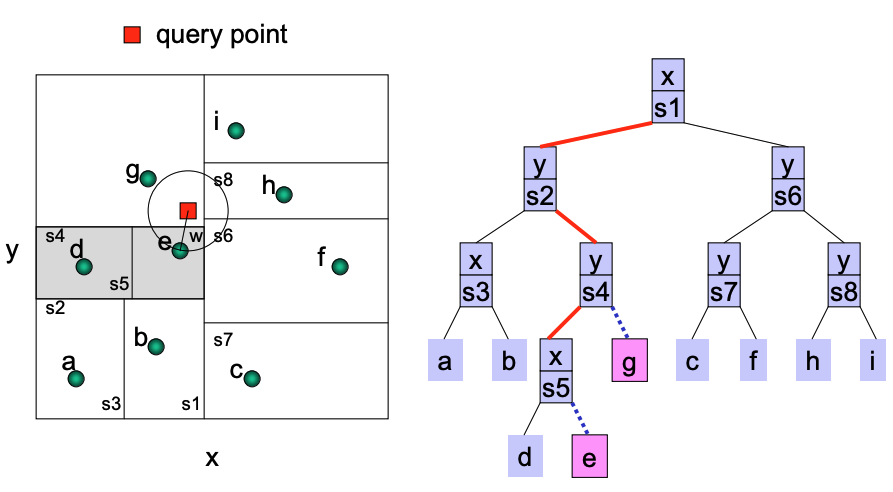
\includegraphics[width=0.8\textwidth]{TheorethicalFramework/ND-Laplace/Images/kd-tree-part2.png}
  \caption{Representation of searching a kd-tree with 2 dimensions \citep{washington_k-d_2002}.}
  \label{fig:kd-tree-searching-theory}
\end{figure}
In the example, we are searching for all points that fall within the radius of a random query point.
The most significant advantage is that this dramatically reduces the complexity of searching.
Constructing the kd-tree costs equal to grid-remapping $O(kn)$, where $k$ is the number of dimensions and $n$ is the dataset size.
But, searching for the nearest neighbor is a logarithmic function with time complexity of $O(\log n)$ \citep{washington_k-d_2002}.
This approach is a significant improvement over searching manually, which would have the same complexity as constructing the tree.

\subsubsection{Grid remapping with kd-tree} \label{theory:grid-remapping}
The kd-tree search method is beneficial for the optimizations we are striving for.
This optimization extends grid-remapping for 2D \citep{DBLP:journals/corr/abs-1212-1984} and 3D data \citep{9646489} to n-dimensions. \newline
We have illustrated the three steps required for this below:
\begin{figure}[H]
  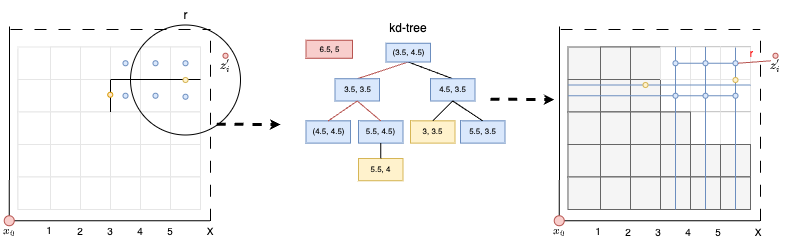
\includegraphics[width=1\textwidth]{TheorethicalFramework/ND-Laplace/Images/KD-tree.png}
  \caption{Representation utilizing a kd-tree for applying grid-remapping \citep{DBLP:journals/corr/abs-1212-1984}}
  \label{fig:kd-tree}
\end{figure}
%When using a kd-tree to search for a data point $z_i$, the algorithm begins with an unbalanced binary tree.
%The root is split by the x-axis, and since 4.5 is greater than 3.5, we go to the right.
%This means that we no longer need to consider the left (greyed out) part of the grid.
%We continue traversing the tree until we find the nearest point based on Euclidean distance.
For easy visualization, the process shown above is with 2-dimensional data.
However, this can be extended to n-dimensional using the kd-tree optimization.
The goal is to remap a perturbed point $z \in Z$, outside the original domain $X$, to the closest point in $X$ or $G$ \citep{DBLP:journals/corr/abs-1212-1984}.

Firstly, a grid is generated, where each (blue) point represents the center of a grid cell.
Together, these centroids form the grid dataset, denoted as $G$.
The yellow points and $x_i$ are part of the original collection, denoted as $X$.
Here, $r$ represents the radius used to generate a private version of the data point $x_i$, named $z_i$, based on 2D-Laplace.
In the illustration, you can observe that $z_i$ falls outside the original domain of $X$, so it needs to be remapped.
We accomplish this by utilizing the nearest-neighbor search from the kd-tree algorithm, allowing us to search in $X \cup G$.
Using this algorithm, we can effectively remap point $z \in Z$ to either $X$ or $G$ based on the closest Euclidean distance (Algorithm \ref{alg:grid-remapping-laplace} and Algorithm \ref{alg:find-outside-domain-laplace}).

A dataset with little dispersion in the data is remapped to the grid regardless of the data shape. 
Generating a grid with sufficiently small grid units to account for this would still result in too much complexity. 
Therefore, in the next chapter, we will look at a variant that addresses this issue.

\begin{algorithm}[H]
  \caption{Algorithm for finding points outside the domain of $X$.}
  \begin{algorithmic}
    \Require $x \in X$  
    \Require $z \in Z$ 
    %\State $tree \gets KDTree(X)$ \Comment construct a KDTree from the original data.
    \State $X_{domain} \gets \Call{KDTree::query}{Z}$ \Comment find the closest points.
    \State $X_{features} \gets \Call{List::getfeatures}{X}$ 
    \State $X_{outside-domain} \gets []$
    \For{$feature \in X_{features}$} 
    \If{$feature \leq \Call{X::min}{Z} $}
    \State $\Call{row::append}{X_{outside-domain}}$
    \EndIf
    \If{$feature \geq \Call{X::max}{Z} $}
    \State $\Call{row::append}{X_{outside-domain}}$
    \EndIf
    \EndFor
    \State \Return $X_{outside-domain}$ 
  \end{algorithmic}
  \label{alg:find-outside-domain-laplace}
\end{algorithm}
\begin{algorithm}[H]
  \caption{Algorithm for generating and remapping to a grid.}
  \begin{algorithmic}
    \Require $x \in X$  \Comment original dataset
    \Require $z \in Z$ \Comment perturbed dataset
    \Require $grid$ \Comment grid structure ($n * m$)
    %\State $tree \gets KDTree(X)$ \Comment construct a KDTree from the original data.
    %\State $X_{domain} \gets$ \Call{KDTree::query}{$Z$} \Comment find the closest points.
    \State $d_{X} = dist(Z, X)$ \Comment euclidean distances
    \State $d_{grid} = dist(Z, grid)$ 
    \State $Z_{out-domain} \gets FindPointsOutsideDomainX(X, Z)$ \Comment Algorithm \ref{alg:find-outside-domain-laplace}
    \State $grid_{tree} \gets KDTree(grid)$ 
    \State $grid_{mask} \gets KDTree::query(Z)$ \Comment find indices of $z \in Z$ that are closeby grid cells.
    \State $Z_{grid-mask} \gets Z_{out-domain} \cup d_{grid} < d_{X}$ \Comment All points $z \in Z$ that are closeby grid cells and are outside domain.
    \State $Z` \gets Z[grid[grid_{mask}][Z_{grid-mask}]]$ \Comment combinate masks to set appropiate indexes to $g \in grid$.
    \State \Return $Z`$
  \end{algorithmic}
  \label{alg:grid-remapping-laplace}
\end{algorithm}
\newpage
\subsection{Density remapping} \label{theory:optimal-remapping}
As discussed, the remapping will be performance intensive to provide good utility, so we adopt the optimal remapping \citep{chatzikokolakis_efficient_2017}.
This thesis will refer to this as density remapping because this better explains the application.

According to the grid-remapping methodology, a private point $z$ is mapped to the center of the grid cell.
The utility is improved by reducing the distance between $z$ and $x$, as this is closer to the original data point.
But, to consider the privacy of the data, this can only be done if there is enough indistinguishability between $z$ and $x$.
To this end, we adopt the remapping approach of Chatzikokolakis et al. to remap based on the data density \citep{chatzikokolakis_efficient_2017}.
The remapping algorithm works on the idea of crowded places, with the intuition that a crowded place leverages indistinguishability by crowdedness (density) \citep{chatzikokolakis_efficient_2017}.  \newline

The approach is visualized using the following figure:
\begin{figure}[H]
  \includesvg{TheorethicalFramework/ND-Laplace/Images/master-thesis-Page-12.svg}
  \label{fig:optimal-remapping}
  \caption{Representation of density remapping \citep{chatzikokolakis_efficient_2017}}
\end{figure}
The first step is calculating $B_r(z)$, which refers to all the data points within the radius $r$ around the data point $z_i$ \citep{chatzikokolakis_efficient_2017}.
Then, the algorithm collects the data points around $x_i$, again using $r$, to determine the density of $x_i$.
This is the convex hull (collection) of all the original data points within the radius $r$ around $x_i$ and is denoted as $Q_r (x)$.
Finally, we obtain $Q_r$ which is a union of $Q_r (x)$ and $B_r(z)$.
Now that we have the sets of points around $x_i$ and $z_i$, we can calculate the density \citep{chatzikokolakis_efficient_2017}:
\begin{equation}
  \forall x' \in Q_r \quad \sigma(x) = \frac{w(x')e^{-\epsilon d(x'_i, z_i)}}{\sum{_{q\in Q_r} w(q)e^{-\epsilon d(q, z)}}}
  \label{eq:optimal-remapping-formula-1}
\end{equation}
$w(q)$ is the weight of a point $q \in Q_r$, and $w(x_i)$ the weight of a point $x_i \in X$.
Here, the weight can be a point of interest \citep{chatzikokolakis_efficient_2017}.
But, in the context of our study, we consider the points within $r$ of $q$ or $x_i$ to be the weight.

In equation \ref{eq:optimal-remapping-formula-1}, the $w(x)$ and $w(q)$ are normalization factors for estimating the likelihood of a point $x'$ being close to $z_i$ and $q$ being close to $z$.
So, this remapping is according to the original definition of the 2D Laplace \gls{pdf} definition \ref{eq:polar-laplace-pdf}.
The outcome of the formula is a collection of values that indicate the degree of density $\sigma(x)$.
The new value $z'$ is calculated by taking the mean of the $\sigma(x)$ \citep{chatzikokolakis_efficient_2017}:
\begin{equation}
  z' = \sum_{x' \in Q_r} \sigma(x') * x'
  \label{eq:optimal-remapping-formula-2}
\end{equation}
By applying this formula, the new $z'$ is closer to $x$ to minimize the expected loss of utility \citep{chatzikokolakis_efficient_2017}.
Much like the 2D and 3D Laplace methods, which use the likelihood of a point $z$ being close to $x$ \citep{DBLP:journals/corr/abs-1212-1984, 9646489}.
%The first step is to calculate the coefficients for each point $x \in X$ by multiplying the density $\sigma(x)$ with the original point $x$.

%The probability that $z'$ will be closer to $x$ is higher, and this probability is calculated based on the original value $x \in X$ to first determine the coefficient.
%Finally, the new $z'$ is calculated by taking the mean value of $\sigma(x)$ \citep{chatzikokolakis_efficient_2017}.
%As described by chatzikokolakis et al., the 
%Chatzikokolakis et al's work considers a prior set of data point $Q \in R^n$.
%Which are other data points that belong to the user.
%We are interested in the data points that are within the radius $r$ around $z$.
%This is denoted as $B_r(z)$, which is the vector of all points within radius $r$ around $z$.
%In addition to this, there is also a $Q_r$ that is a convex hull of all nearby points.
%Hence, this is described as $Q_r = B_r \cap Q$.
%The final intuition here is that $r$ is automatically generated based on crowdedness (see circle inside figure \ref{fig:optimal-remapping}).
%The last step is to take the mean value of $\sigma(x)$.
%Unfortunately, optimal remapping is not possible for users that do not have sufficient data (e.g. new users).
%The remapping is not applied for these users and is also not applied for $z$ if it is within the domain of $X$.
\begin{algorithm}[H]
  \caption{Algorithm to implement the density remapping of $z \in Z$ to be in the domain of $x \in X$}
  \begin{algorithmic}[1]
    \Require $x \in X$
    \Require $z \in Z$
    \Require $epsilon$
    \Ensure $z' \in Z$
    \State $Z' = FindRemappedPoints(Z)$ \Comment Algorithm: \ref{alg:find-outside-domain-laplace}
    \State $tree \gets KDTree(X)$
    \For{$z' \in Z'$}
    \State $r = \Call{FindRadius}{(z')}$ \Comment Get original radius $r$.
    \State $X_r \gets \Call{KDTree::query}{x}$ \Comment find $q \in X$ around $x$ with radius $r$.
    \State $B_r \gets \Call{KDTree::query}{z'} $
    \State $\sigma(x) = []$
    \State $Q_r = \gets X_r \cap B_r$
    \State $w_x = \Call{Length}{X_r, B_r}$ \Comment weight is simply adding density of $X_r$ and $B_r$.
    \For{$q \in Q_r$}
    \State $q \gets \Call{KDTree::query}{q}$
    \State $w_q = \Call{Length}{Q_r}$ \Comment $w_q$ is the density of each point $q$ within $Q_r$.
    \State $\sigma(w_x) \gets \Call{Remap}{w_x, \epsilon}$ \Comment Equation \ref{eq:optimal-remapping-formula-1}.
    \State $\sigma(x) \gets \Call{Append}{\sigma}$ \Comment add to the list $\sigma(x)$.
    \EndFor
    \State $z' \gets \Call{Average}{\sigma(x)}$ \Comment Equation: \ref{eq:optimal-remapping-formula-2}.
    \EndFor
  \end{algorithmic}
  \label{alg:optimal-remapping-laplace}
\end{algorithm}

\begin{itemize}
  \item 1: Receives all the points $z \in Z$ that are outside the domain of $X$.
  \item 2: Constructs a KDTree from the original data $X$, so it can be queried.
  \item 3: Receives the original privacy radius $r$ that was used to generate $z$ from $x$.
  \item 4: $X_r$ is the set of points $x \in X$ that are within the radius $r$ of $x$.
  \item 5: $B_r$ is the set of points $z \in Z$ that are within the radius $r$ of $z$.
  \item 7: $w_x$ is the "popularity" of $x$ and $z$, for the number of points is counted within the radius $r$.
  \item 12: $w_q$ is the weight of each point $q \in Q_r$, so $q$ is re-assigned to be the number of points within the radius $r$ of $q$.
\end{itemize}

\newpage
The equation for density remapping \ref{eq:optimal-remapping-formula-1} was created for 2-dimensional data.
However, we aim to use this same approach for 3-dimensional and n-dimensional data.
To do so, we first revisit the \gls{pdf} for 3D-Laplace, which was defined using this Equation: \ref{eq:3d-laplace-pdf}.
Few modifications are necessary, as the normalization factor $A$ is now defined using Equation: \ref{eq:optimal-remapping-formula-1}.
\todo[inline]{Formulate the definition of $A$}
\todo[inline]{Check if this can be extended to nD-Laplace}

\newpage
\subsection{Putting it together: nD-Laplace}
Now that we have defined everything, we can write the algorithm in a step-by-step manner:
\begin{algorithm}[H]
    \caption{Full algorithm for perturbing training data for nD-clustering using planar/2D-Laplace \citep{DBLP:journals/corr/abs-1212-1984}}\label{alg:rq1}
    \begin{algorithmic}
      \Require $x \in X$  \Comment 2D array of points
      \Require $l \in R^ +$
      
      \State \Return Z
    \end{algorithmic}
    \label{alg:nd-laplace}
  \end{algorithm}

It is important to note that with the introduction of this algorithm, it is no longer a non-interactive method, as the data points now interact with each other.
Due to the extra interaction rounds, we expect the introduction of density grid remapping with kd-tree will bring more utility \citep{wang_comprehensive_2020, xiongComprehensiveSurveyLocal2020}.
If this proofs to be true, it might out-weights the privacy implications for clustering.
%\todo[inline]{Also refactor this}

%\subsection{Extending to $d_x$-privacy}
%\todo[inline]{Find if this is possible}

%Constructing elastic distinguishability metrics for location privacy
\newpage

\subsection{Mechanism flowchart}
All formulas and theories are established for 2D, 3D, and nD-Laplace, so the mechanism design applies to all three variants:
\begin{figure}[h]
  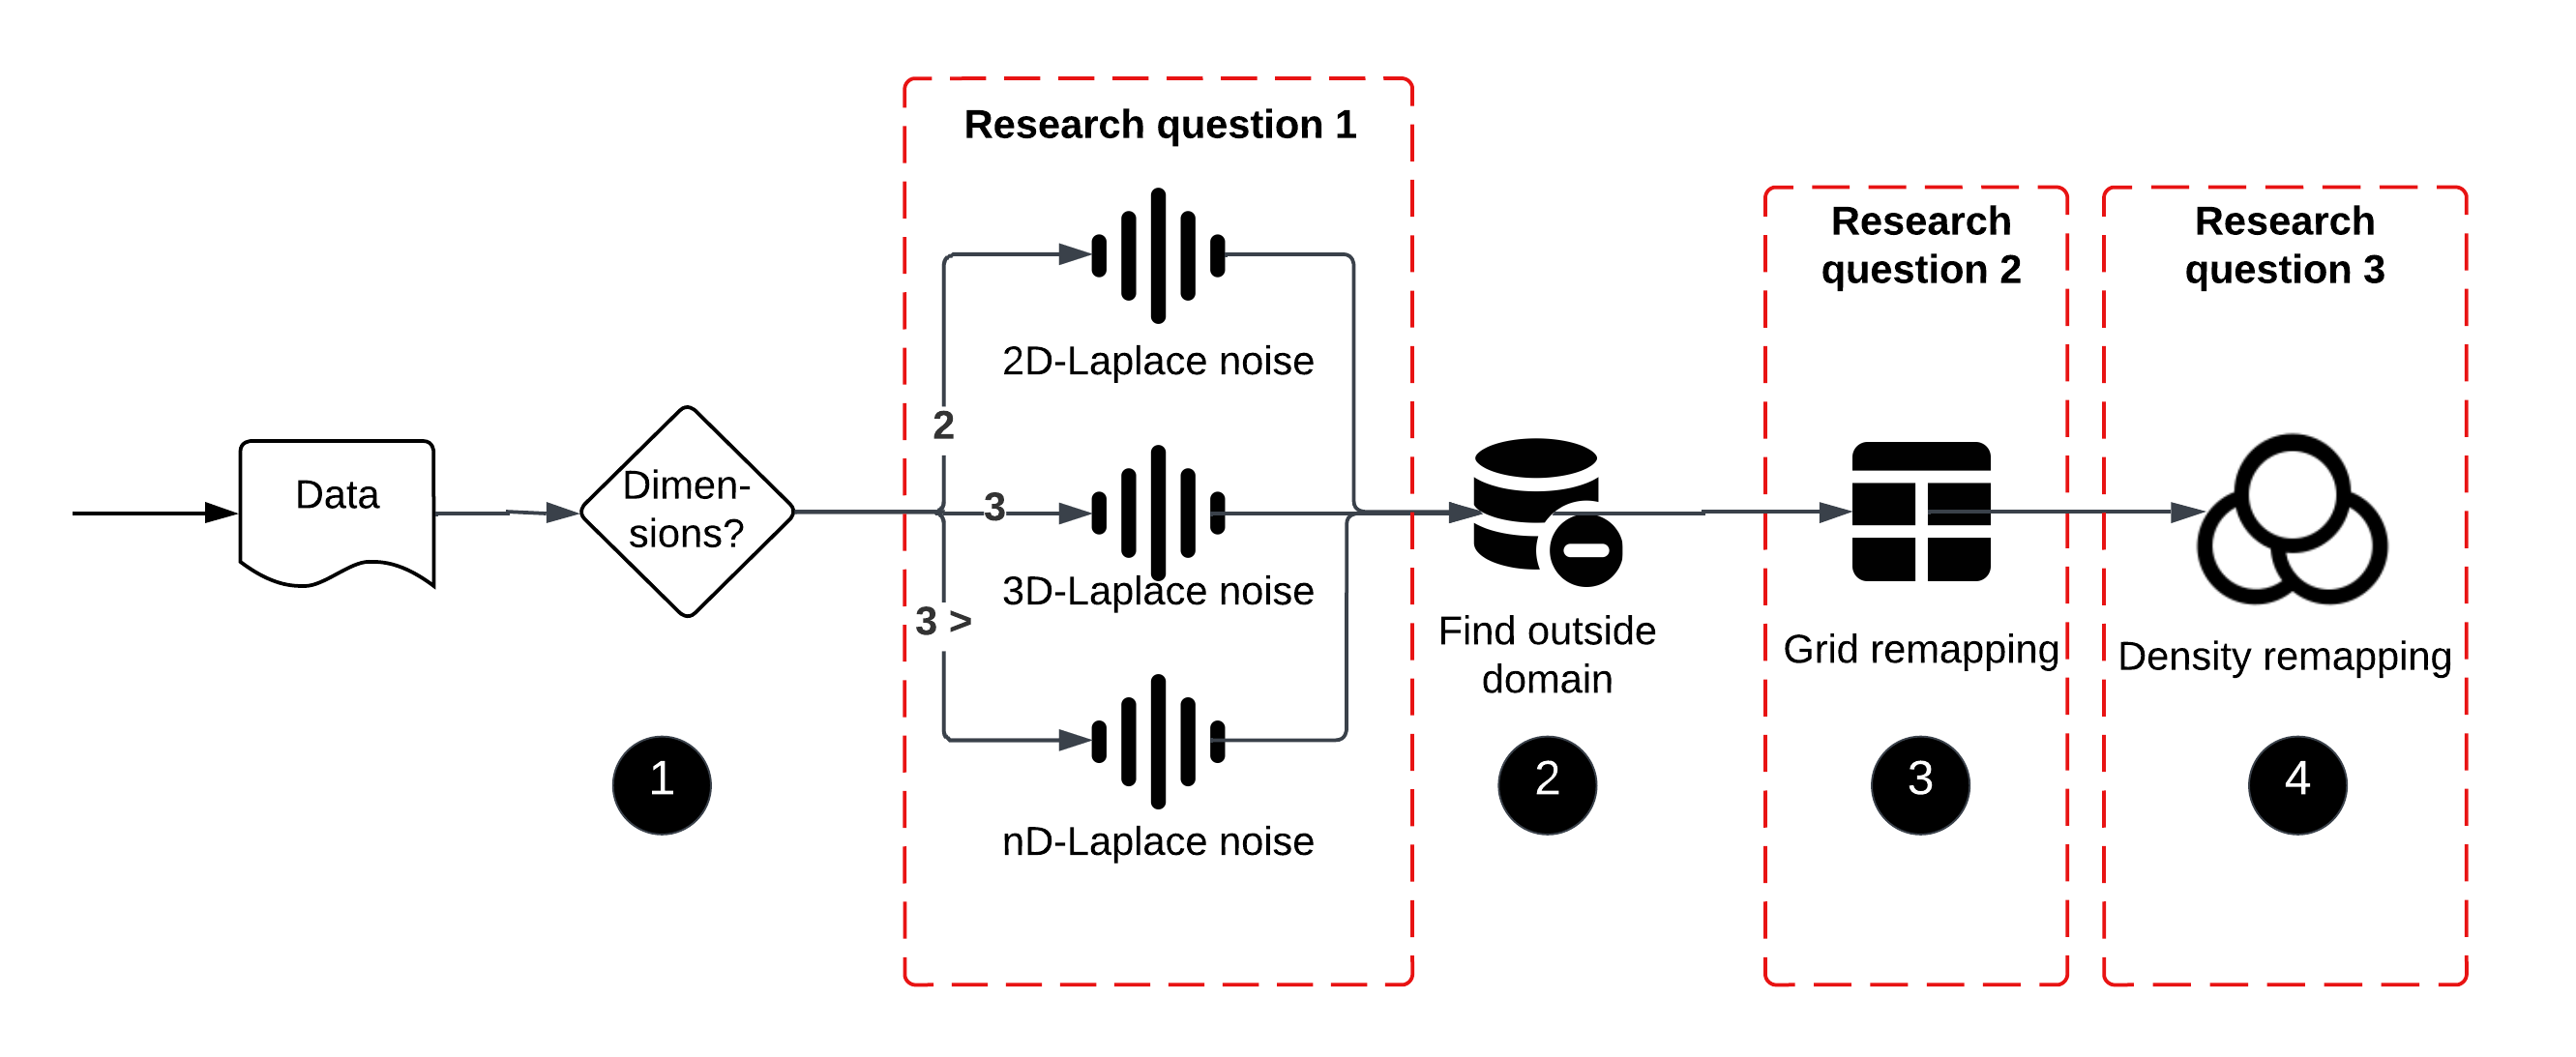
\includegraphics[width=1.1\textwidth]{TheorethicalFramework//ND-Laplace//Images/Thesis-nd - final-mechanism-design.png}
  \caption{Non-interactive mechanism design for nD-Laplace.}
  \label{fig:final-mechanism-design}
\end{figure}
%\todo[inline]{Modify to density-nD-Laplace \& nD-Laplace for image reporting}
For easy navigation, we provide a list of all algorithms:
\begin{enumerate}
  \item Based on the number of dimensions, the algorithm decides the correct Laplace mechanism to use:
        \begin{itemize}
          \item 2D-Laplace:  \ref{alg:2d-laplace}
          \item 3D-Laplace: \ref{alg:3d-laplace}
          \item nD-Laplace: \ref{alg:nd-laplace}
        \end{itemize}
  \item Find points outside domain: \ref{alg:find-outside-domain-laplace}
  \item Grid remapping: \ref{alg:grid-remapping-laplace}
  \item Density remapping: \ref{alg:optimal-remapping-laplace}
\end{enumerate}
\added{In addition, relevant research questions are incorporated into the architecture overview.
These questions are covered in chapter \ref{chapter:methodology}}.
\subsubsection{Practical example}
The shape of the dataset is necessary for the usefulness of clustering.
With our algorithm, there are four different shapes/variants of the dataset.
For example, this has been visualized using a 3D dataset based on the heart dataset (\ref{datasets-section}).
Our mechanism aims to provide privacy and preserve the dataset's shape to benefit the utility of clustering.
Grid remapping and optimal remapping are used to achieve this goal.

\begin{figure}[H]
  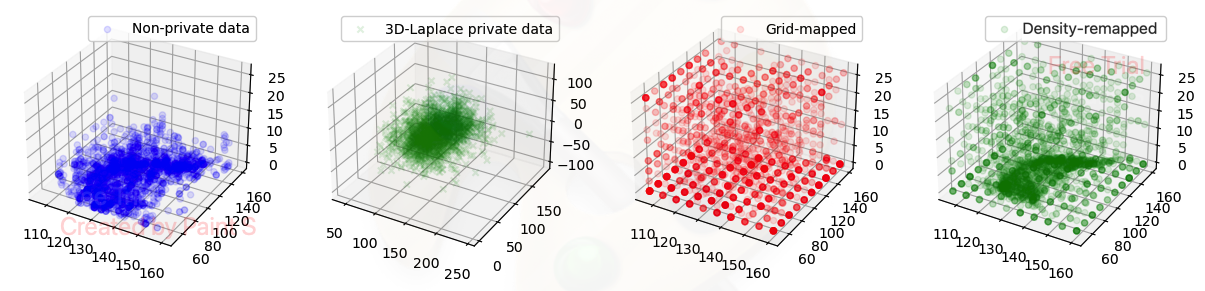
\includegraphics[width=1.1\textwidth]{TheorethicalFramework/ND-Laplace/Images/optimal-remapping-example.png}
  \caption{Example of optimal remapping for the 3D-dataset: Cardiotocography. The example shows the different steps of the mechanism in sequence for a dataset perturbed with a privacy budget of 0.1.}
\end{figure}

\begin{enumerate}
  \item Dataset: the blue dots represent the original dataset without any modifications.
  \item Adding noise: the green crosses represent the dataset after adding noise; for this particular example, this is 3D-Laplace (Algorithm \ref{alg:3d-laplace}):
        As can be observed, the data is generated from the center, causing many data points to fall outside the original domain of the dataset.
  \item Grid-remapping: the red dots represent the dataset after grid-remapping (Algorithm \ref{alg:grid-remapping-laplace})
        After performing the grid remapping algorithm, all points within the domain are plotted.
        However, the original shape of the data is mostly lost.
        This makes it challenging to cluster the data as was possible with the original data.
  \item Optimal-remapping: the green dots represent the dataset after optimal-remapping (Algorithm \ref{alg:optimal-remapping-laplace}).
        After completing the previous step, the data points are again remapped based on the (original) density.
        This results in restoring the original shape of the data and, consequently, the clusters.
\end{enumerate}

